\subsection{Long Baseline - M Wilking for LBL group}
%\paragraph{Motivation}
%BRIEF intro to physics motivation, and status of the field: our major competitors
%\paragraph{XX with THEIA}
%What we bring to the table - pros of THEIA design \newline
%Sensitivity estimates with baseline design (one of THEIA i--iii)
%\paragraph{Detector Requirements}
%A summary of the impact of different detector choices i.e. what happens if we stray from the relevant baseline

%How much do we want here?
ETW note: Basically just copied in text from proposal - will need to be expanded.

Neutrino oscillation arises from mixing among the flavor and mass states of the neutrino that is described
by a complex unitary matrix that depends on three mixing angles and a potentially CP-violating phase. The
parameters of this PMNS matrix determine the probability amplitudes of neutrino oscillation and the
differences between the neutrino masses determine the frequency of oscillation. These parameters have
all been measured, with the exception of the value of the CP-violating phase, $\delta_{CP}$ and the ordering
of the mass states. Long-baseline neutrino oscillation experiments have signficant sensitivity to the
mixing parameters $\theta_{23}$, $\theta_{13}$, and $\delta_{CP}$, as well as to the mass splitting
$\Delta m^{2}_{32}$, and the neutrino mass ordering via matter effects. [Some comment on existing experiments]
DUNE is a next-generation long-baseline neutrino oscillation experiment that will make a definitive
determination of the neutrino mass ordering, will have sensitivity for a definitive discovery of CP-violation
for much of the possible parameter space, and will make precise measurements of all the oscillation
parameters governing long-baseline oscillation in a single experiment.
Theia will be able to supplement the DUNE measurements with CP-violation sensitivity comparable to a
10-kton liquid argon detector.

The presence of an additional detector at LBNF that can measure long-baseline neutrino oscillations with an
entirely separate set of detector systematic uncertainties and neutrino interaction uncertainties than
DUNE would constitute a substantial upgrade to the physics reach of the currently envisioned program.
Of course, such a detector must be able to achieve a sensitivity comparable to that of a 10-kton DUNE liquid
argon detector, such that the DUNE projections\cite{DUNECDR} based on 40-kt of far detector mass can be achieved.
For the study presented here, we use GLoBES\cite{globes} to calculate predicted spectra for different
oscillation parameter hypotheses and compare these to quantify experimental sensitivity. We make use of
the publicly available LBNF beam flux and DUNE detector performance description\cite{DUNE_configs}. For the DUNE
sensitivity we assume a 10 kton fiducial mass, corresponding to a single DUNE far detector module. For the
Theia sensitivity, we use Theia’s expected 17-kton fiducial mass and very conservatively assume the detector
can be designed to perform as well as and no better than a conventional water Cerenkov detector (WCD), using
Monte Carlo simulations from Super Kamiokande to define this performance. Detailed simulations of improved
performance from using LAPPDs, WbLS, and advanced image recognition algorithms are planned and expected to
demonstrate improved performance. Consistent with DUNE, we assume seven years exposure with equal running
in neutrino and
antineutrino mode for both detectors, and use oscillation parameter central values and uncertainties
from NuFit 4.0\cite{nufit4}.

Previous studies of a water Cherenkov detector in the LBNF beam were performed in the context of the
predecessor experiment to DUNE: LBNE\cite{lbne}. These studies were based on Super-K event reconstruction techniques
developed within the first several years of Super-K data taking, and were restricted to single- ring events with
no Michel electrons from stopped pion and muon decay. In the decade since, important advancements have been made in
Cherenkov reconstruction that have substantially improved particle identification and ring counting, which have
now been fully implemented in the most recent T2K analyses\cite{t2k}. These improvements, when applied to the
new, lower energy LBNF beam, enhance the sensitivity to neutrino oscillations in three important ways: (1)
The improved ring counting has removed 75\% of the neutral current background, relative to the previous analysis,
due to improvements in the detection of the faint second ring in boosted $\pi^{0}$ decays;
(2) The improved electron/muon
particle identification has allowed for an additional sample of 1-ring, zero Michel electron events
from $\nu_{3}$-CC$\pi^{+}$ interactions, without significant contamination from $\nu_{\mu}$ backgrounds; (3)
Multi-ring $\nu_{e}$ event samples can now be selected with sufficient purity to further enhance sensitivity to
neutrino oscillation parameters.

The long-baseline oscillation analysis now includes nine samples that are analyzed with independent systematic
uncertainties within a single fit: one, two-, and three-ring events with either zero or one Michel electron
in neutrino mode, and the corresponding zero Michel electron samples for anti-neutrino mode. As an example,
spectra for the one-ring-zero-decay and one-ring-one-decay samples are shown in \ref{fig:lblspectra}. The two-
and three-ring samples tend to have higher background than the single-ring samples, but do make significant
contributions to the overall sensitivity.

\begin{figure}[h!]
  \centering
  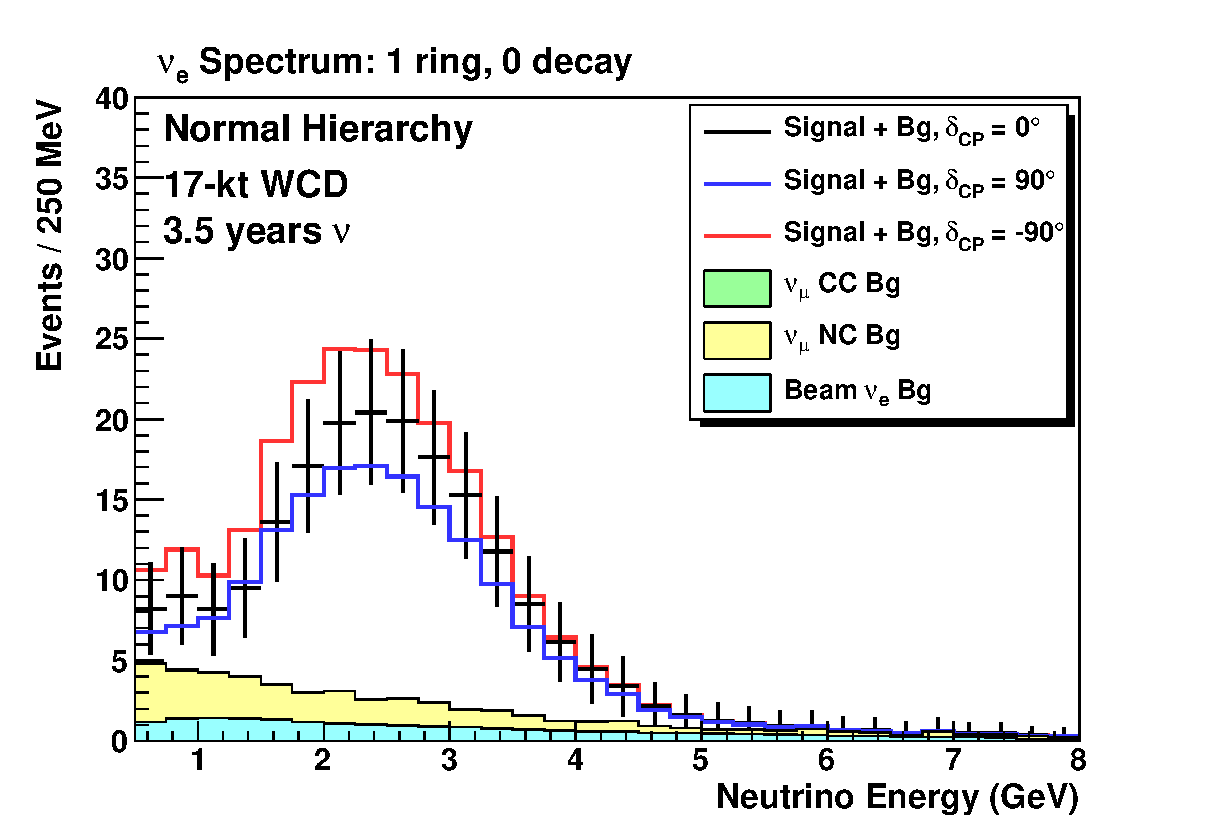
\includegraphics[width=0.3\linewidth]{lbl/nu_water_skfq_1ring0decay_normal.eps}
  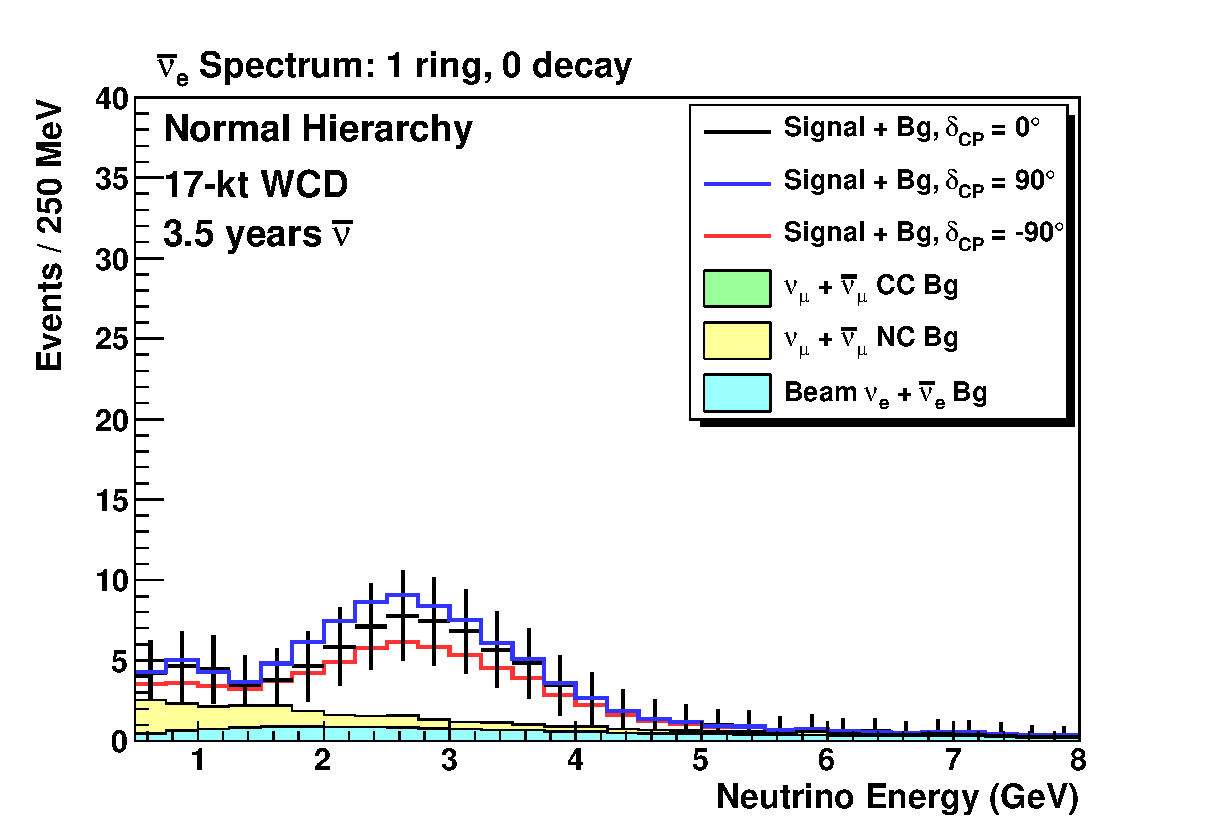
\includegraphics[width=0.3\linewidth]{lbl/anu_water_skfq_1ring0decay_normal.eps}
  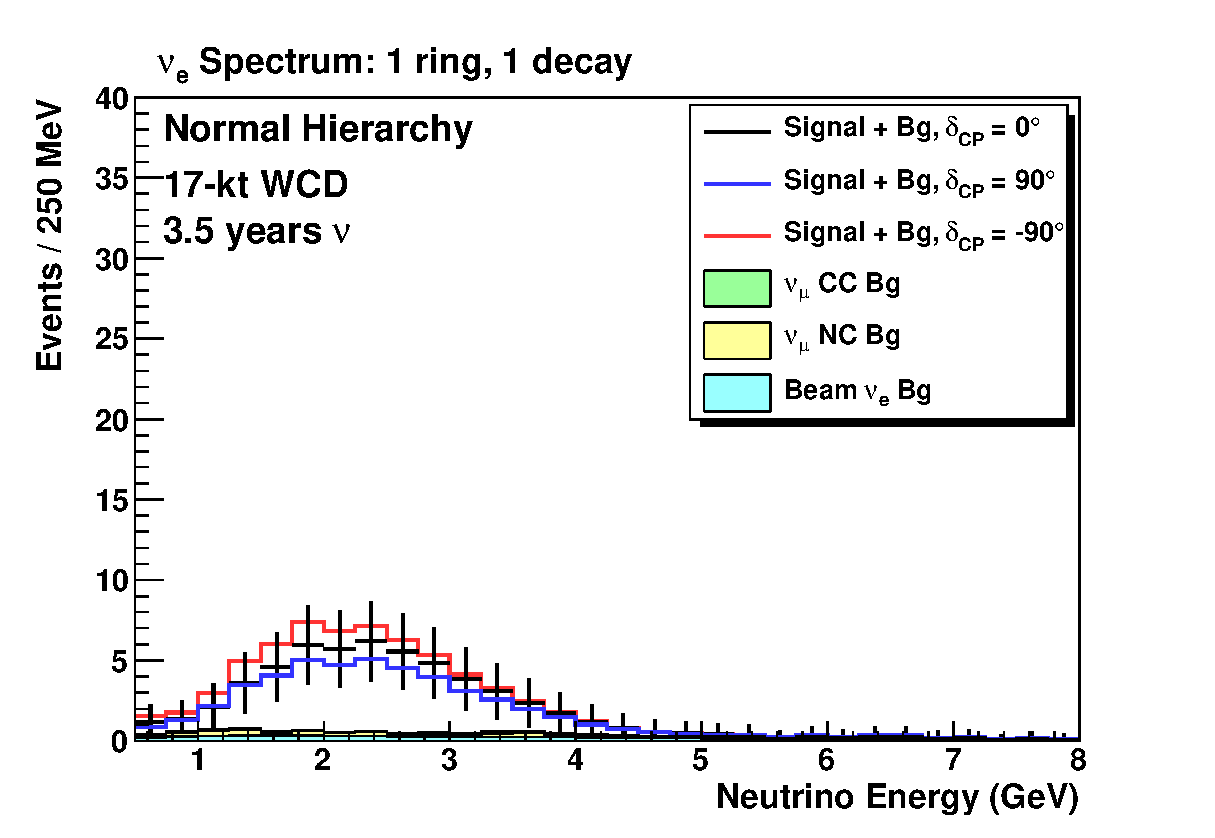
\includegraphics[width=0.3\linewidth]{lbl/nu_water_skfq_1ring1decay_normal.eps}
  \caption{Expected event rates as a function of reconstructed neutrino energy for Theia after 7 years in the LBNF beam. Left: neutrino mode 1-ring+0-decay; Middle: antineutrino mode 1-ring+0-decay; Right: neutrino mode 1-ring+1-decay. The corresponding two and three ring samples are not shown.}
  \label{fig:lblspectra}
\end{figure}

We assign independent normalization uncertainties of 2\%(5\%) on the $\nu_{e}$ and $\overline{\nu}_{e}$ appearance
signal(background). We do not explicitly include the $\nu_{\mu}$ disappearance samples, but the choice of
uncertainty for the appearance samples assumes some systematics constraint from the disappearance samples.
This treatment of systematic uncertainty is comparable to that in the DUNE CDR analysis. We find the sensitivity
of the 17-kt WCD to be comparable that of the DUNE 10-kt LArTPC, as shown in Fig.~\ref{fig:lbl17kt}.
It is expected that this will improve when the modern fast HQE PMTs, WbLS, and LAPPDs are considered. 

\begin{figure}[h!]
  \centering
  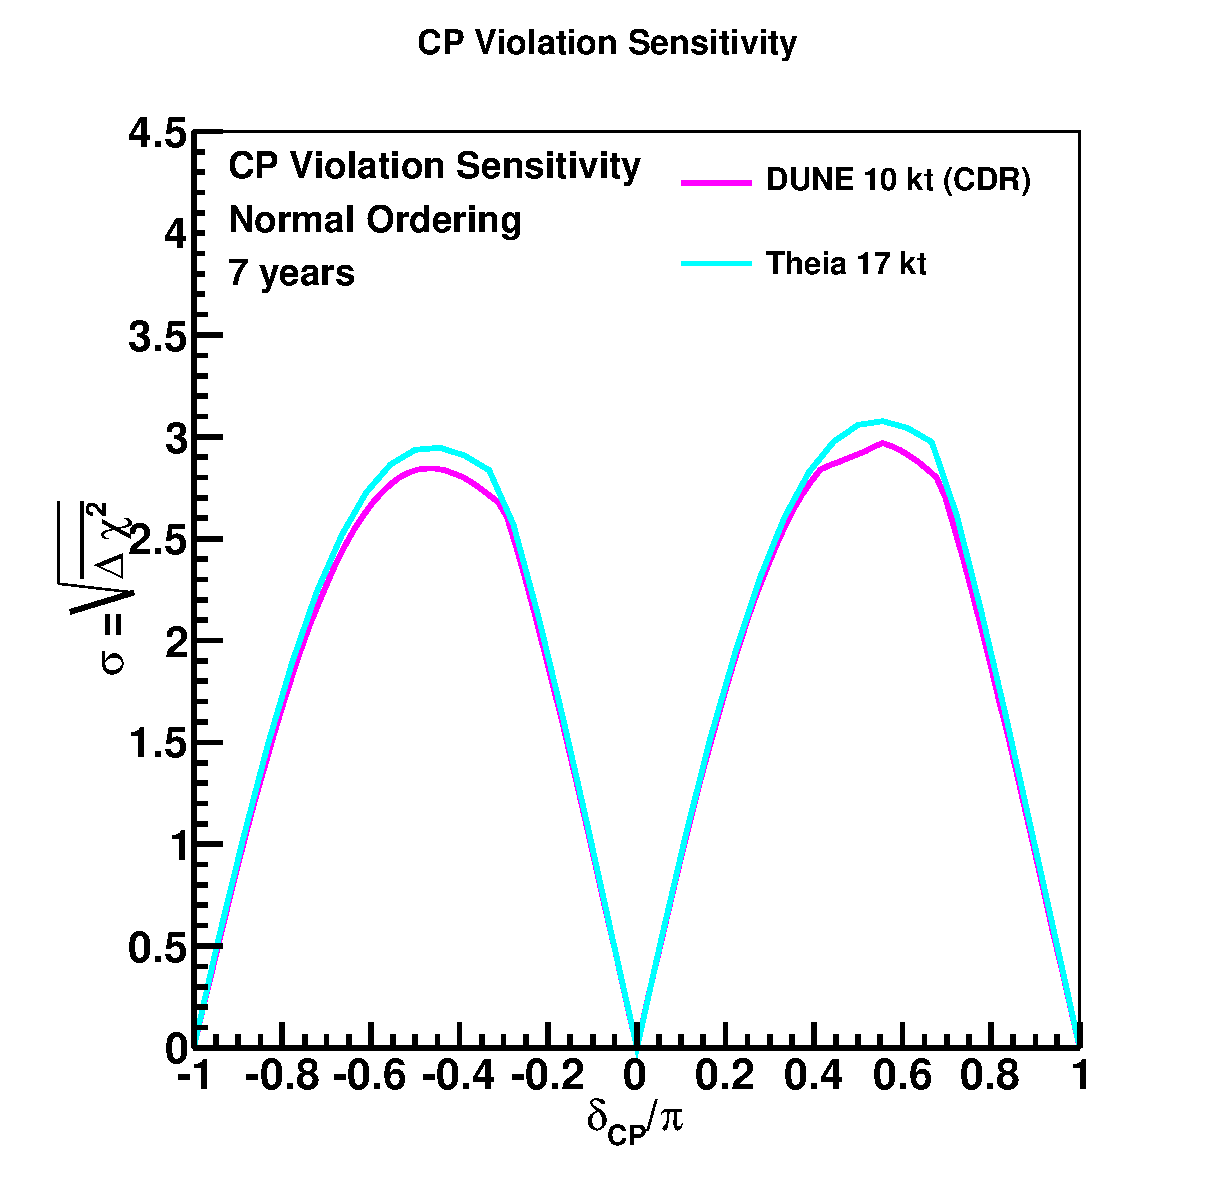
\includegraphics[width=0.45\linewidth]{lbl/cpv_theia_17kt.eps}
  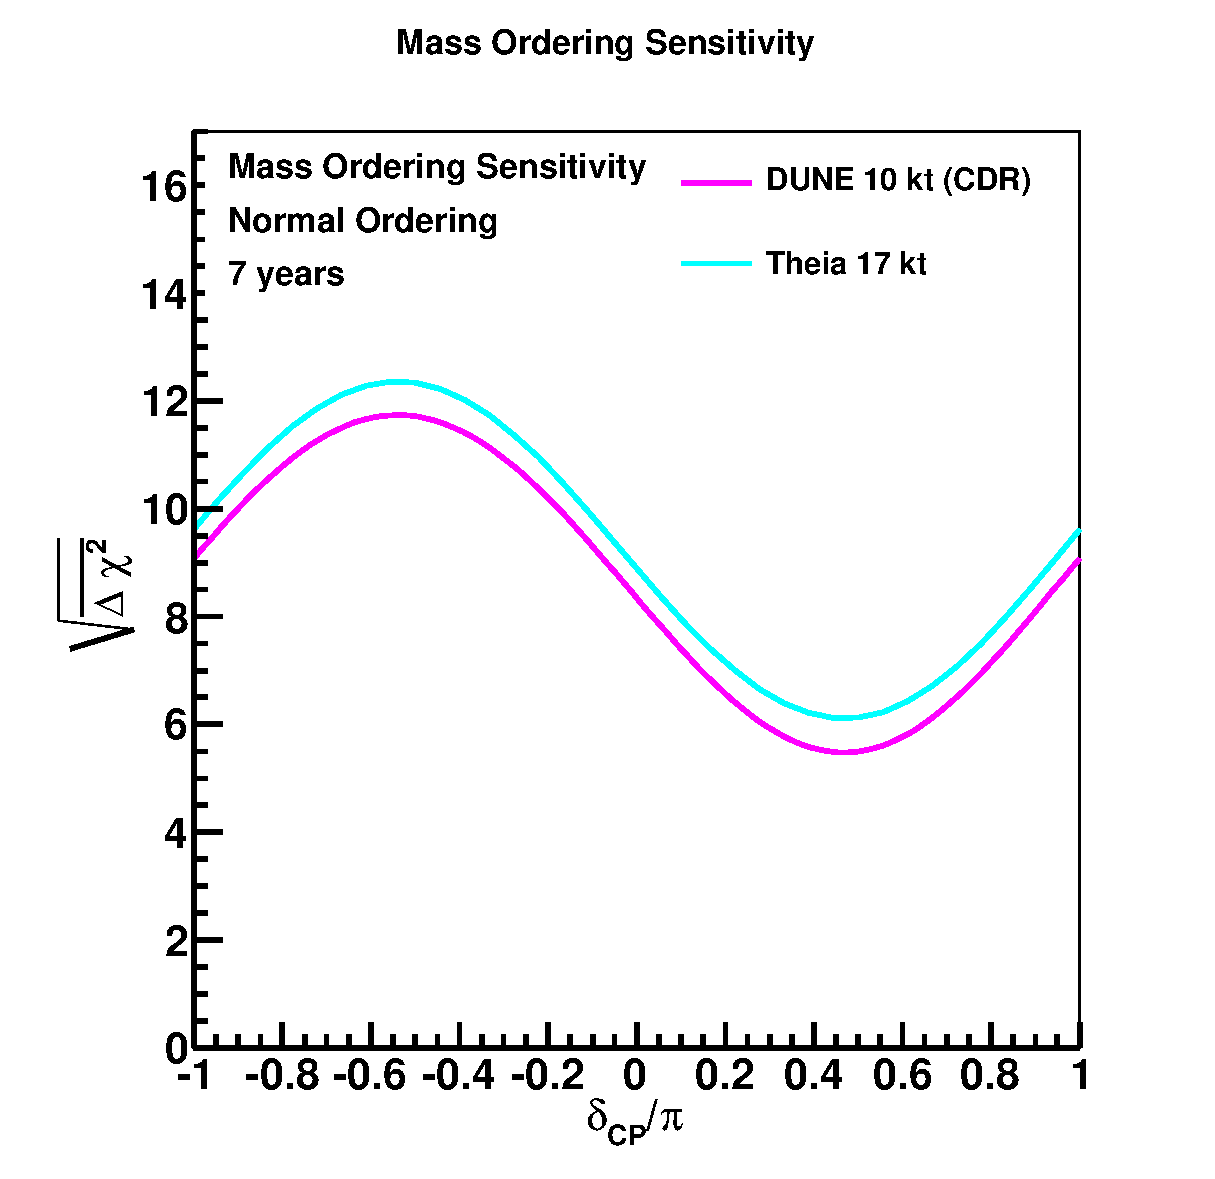
\includegraphics[width=0.45\linewidth]{lbl/mh_theia_17kt.eps}
  \caption{Sensitivity to CP violation (i.e.: determination that $\delta_{CP} \ne$ 0 or $\pi$) (left) and sensitivity
    to determination of the neutrino mass ordering (right), as a function of the true value of $\delta_{CP}$, for
    a 10-kt LArTPC (pink) compared to a 17-kt WCD (blue). Seven years of exposure to the LBNF beam
    with equal running in neutrino and antineutrino mode is assumed. LArTPC sensitivity is based on
    detector performance described by \cite{DUNEconfigs}.}
  \label{fig:lbl17kt}
\end{figure}

